\definecolor{shell_default}{HTML}{e4e4e4}
\definecolor{shell_background}{HTML}{272a36}
\definecolor{shell_command}{HTML}{59f68e}
\definecolor{shell_quote}{HTML}{f4f89d}
\definecolor{shell_variable}{HTML}{ff93d0}
\definecolor{shell_file}{HTML}{99ecfe}
\definecolor{shell_operator}{HTML}{c9a8fb}
\definecolor{shell_escape}{HTML}{99ecfd}

\lstset{
    literate={~} {$\sim$}{1}
}

\def\shellquote{\textcolor{shell_escape}{\texttt{\string\"}}}
\def\shellrawquote{\textcolor{shell_default}{\texttt{"}}}

\lstdefinestyle{ShellInputStyle}{
  language=bash,
  basicstyle=\small\sffamily\ttfamily,%
  numbersep=3pt,
  frame=tb,
  columns=fullflexible,
  backgroundcolor=\color{shell_background},
moredelim=**[is][\color{shell_variable}]{@}{@},
moredelim=**[is][\color{shell_operator}]{+}{+},
moredelim=**[is][\color{shell_file}]{§}{§},
moredelim=**[is][\color{shell_command}]{!}{!},
moredelim=**[is][\color{shell_quote}]{\%}{\%},
moredelim=**[is][\bfseries]{^}{^},
linewidth=0.95\linewidth,
  xleftmargin=0.1\linewidth,
  stringstyle=\color{shell_quote},
keywordstyle=\color{shell_command},
moredelim = [s][\color{purple}]{\\[}{\\]},
morekeywords={run, time, wc, tee},
basicstyle=\footnotesize\ttfamily\color{shell_default},
morestring=*[d]{"},
morestring=[s][]{\#\{}{\}},
escapeinside={\%*}{*}
}


\chapter[Shell]{Shell \\ \Large \textnormal{Jan Luca Scheerer}}
\label{chapter:shell}

The shell plays a crucial role in the functionality and versatility of any operating system. Acting as the bridge between the user and the underlying system, the shell provides a powerful interface for executing commands, managing processes, and manipulating files and directories. 

In this chapter, we delve into the milestones of enhancing the UART driver and implementing essential features of the shell. We begin by covering the extension of the UART driver, followed by a detailed discussion on the core functionality of the shell. This functionality includes syntax highlighting, tab completion, and the ability to define custom session variables.

To further explore the capabilities of the shell, we conclude this chapter by examining its advanced features. These features include support for executing lists of commands and command pipelines, enabling both I/O redirection and pipes.

\section{Userspace UART Driver}

As outlined in Chapter \ref{chapter:mp}, all RPC services are coordinated by each core's respective init process, and potentially forwarded to a different core's init process, if the request cannot be completed \emph{locally}. The userspace UART driver conforms to this paradigm: it runs as part of \texttt{init.0}, and any serial request addressed to a different core's init process will relay the request to \texttt{core 0}.

The driver is set up following the guidelines and instructions provided in the relevant section of the AOS Book. First, we initialize the GIC distributor driver by mapping the GIC to the current address space and calling \texttt{gic\_dist\_init}. Next, we initialize the \texttt{LPUART} driver by once again mapping the corresponding device frame into our address space and calling the appropriate initialization function - \texttt{lpuart\_init}. Having initialized both the GIC distributor and the \texttt{LPUART} drivers, we can now allocate a new IRQ destination capability and attach our handler via calls to \texttt{inthandler\_alloc\_dest\_irq\_cap} and \texttt{inthandler\_setup} respectively. Finally, we call \texttt{lpuart\_enable\_interrupt} to enable interrupts in the \texttt{LPUART} and conclude the initialization.

To provide a similar experience, whether the operating system is run on \texttt{QEMU} or on the Toradex board, our serial driver implements an adapter pattern: based on the platform provided to \texttt{serial\_server\_init}, the server either initializes the \texttt{LPUART} driver and utilizes the constants defined in \texttt{imx8x\_map.h} as described above, or it makes use of the \texttt{PL011} UART driver and the constants defined as part of \texttt{qemu\_map.h}. As both interfaces are effectively identical, the serial driver needs only to call the function appropriate for the current platform with the relevant constants. Throughout the code any reference to a platform specific constant is, therefore, encapsulated behind a \emph{generic} function (e.g., Listing \ref{listing:shell_serial_adapter}).

\begin{lstlisting}[caption={Serial Driver: Platform Independent UART Base},label={listing:shell_serial_adapter}]
static genpaddr_t _platform_uart_base(struct serial_state *state)
{
    switch (state->platform) {
    case PI_PLATFORM_QEMU:
        return QEMU_UART_BASE;
    case PI_PLATFORM_IMX8X:
        return IMX8X_UART3_BASE;
    default:
        __builtin_unreachable();
    }
}
\end{lstlisting}

The implementation as an adapter means that the serial server can provide a unified interface regardless of the concrete platform the operating system is running on. The server's interface beyond initialization is depicted in Listing \ref{listing:shell_serial_interface}\footnote{Additionally, the server allows checking if the platform provided during initialization is known, i.e., is either \texttt{QEMU} or \texttt{IMX8X}, via \texttt{is\_usr\_serial\_enabled}. This allows us to fall back to the syscall in the corresponding rpc call in case of an unknown platform.}$^{,}$\footnote{The server also provides the option to output a single character via \texttt{serial\_putchar}.}.

\begin{lstlisting}[caption={Serial Driver: UART Interface},label={listing:shell_serial_interface}]
errval_t serial_putstr(const char *buf, size_t len,
											 size_t *retlen);

errval_t serial_getchar_register_wait(size_t len, struct event_closure resume_fn, size_t *retlen, char *buf);
\end{lstlisting}

In the following sections, we will discuss the design and implementation of both functions.

\subsection{Writing via UART}

As \texttt{serial\_putstr} will be called as part of the corresponding libc function set in \texttt{\_libc\_terminal\_write\_func}, its signature closely resembles the one expected by the libc endpoint. In essence, \texttt{serial\_putstr} iterates over the provided buffer and calls the corresponding uart driver function. Similar to the way platform specific constants are handled by the serial server, platform specific calls to uart putstr are encapsulated behind a generic \texttt{\_platform\_putchar} function. In contrast to reading, writing via the UART is implemented as a blocking call. Additionally, writes are performed consecutively. Thus, multiplexing of writes is not a concern. If this is desired, it is possible to e.g., implement an upper limit for the size of the provided buffer, or to consider a write as completed, once a new line character is emitted.

\subsection{Reading via UART} \label{sec:shell_read_uart}

Reading via UART is substantially more difficult to implement than writing. First, we must set up UART to accept interrupts as previously outlined. Next, the call to the corresponding read function \texttt{serial\_getchar\_register\_wait} must return immediately, as this function will be called as part of handling the corresponding rpc request in init, which may never block (see Chapter \ref{chapter:mp} for more details)\footnote{Note that this does NOT imply that the corresponding \texttt{aos\_rpc} request is non-blocking. Indeed, it is implemented as a blocking call.}.

To address these challenges, \texttt{serial\_getchar\_register\_wait} simply appends the request to a queue of pending \texttt{requests}. Once our designated interrupt handler, \texttt{\_uart\_interrupt}, is called as part of an interrupt, it reads any pending characters and appends them to the buffer at the head of the requests' queue. Once a pending read request is completed, i.e., \texttt{len} characters have been read, the request is removed from the queue and its \texttt{resume\_fn} is invoked. In turn, this triggers that the pending response is sent to the original \texttt{aos\_rpc} request via \texttt{async\_respond}. If the interrupt handler is invoked while no requests are pending, all pending characters will be read and appended to an internal ring buffer, and in turn used to satisfy future requests. Once the ring buffer reaches capacity, it will start to discard previously read characters.

Input multiplexing is performed in a straightforward fashion, building upon the outlined approach. In addition to considering a request as completed once \texttt{len} characters have been read, reading a newline character immediately triggers a request's completion. By issuing large enough read requests, we effectively obtain input multiplexing on a line-by-line basis. In particular, this approach fits great with libc which issues large (e.g., $1024$ byte) read requests, and expects them to return prematurely, if no data is available. The process of enqueuing, processing and finalizing a \texttt{serial\_getchar\_request} is depicted in Figure \ref{fig:serial_read}.

\begin{figure}[htp]
    \centering
    \includegraphics[width=12cm]{images/serial/serial_read.png}
    \caption{Lifetime of a \texttt{serial\_getchar\_request}}
    \label{fig:serial_read}
\end{figure}

\subsection{I/O via RPC} \label{sec:shell_io_via_rpc}

Any serial RPC calls will eventually be processed by the init process of core 0 as outlined in the introduction, potentially being relayed in case the caller is being executed on any other core. Here, the methods outlined in Listing \ref{listing:shell_serial_interface} serve as the basis for the implementation. In addition to supporting the required \texttt{aos\_rpc\_serial\_getchar}  and \texttt{aos\_rpc\_serial\_putchar} procedures, the terminal server allows the caller to read/write entire buffers using the corresponding \texttt{*\_str} functions. As the serial driver infrastructure is set up to support buffers by default, the character specific versions can be considered special cases of the more general buffer methods.

In case the serial driver was initialized with an unknown platform, the RPC calls fall back to the appropriate syscalls bypassing the need to relay to core 0. As outlined in Section \ref{sec:shell_read_uart}, \texttt{serial\_getchar\_register\_wait} is non-blocking. As previously discussed, this is required as the init process is not allowed to block in our implementation.

\subsection{Testing the Serial Server}

We evaluate the functionality of our serial server implementation by using a user process named \texttt{serial\_tester}. Initially, the \texttt{serial\_tester} performs a sequence of write operations and subsequently performs a variable number of read operations. By spawning a single instance of the \texttt{serial\_tester}, we can test the fundamental features of the serial server. However, to examine potential interleaving and ensure accurate line-based multiplexing, we spawn multiple processes for testing purposes\footnote{We can spawn multiple \texttt{serial\_tester} processes by providing the desired number of processes to spawn as a command line argument: \texttt{run serial\_tester [num\_procs]}}.

\section{Command-Line Interface}


Having discussed the technical underpinnings, we can now discuss the implementation of the shell. The shell implements a command-line interface by reading a single character at a time\footnote{A line based approach would be insufficient to support tab-competition and syntax highlighting effectively.}, tokenizing it, and finally interpreting the command. The following section covers the entire process roughly in this order, before examining the more advanced features (i.e., the extra challenge) in subsection \ref{sec:shell_pipes_and_io}. 

\subsection{Reading a Line}

The \textbf{entire code was written from scratch} as part of this project, although porting the \texttt{readline} code from the FreeBSD library or more lightweight alternatives such as \href{https://github.com/antirez/linenoise}{\texttt{linenoise}} would have been considerably more straightforward. In particular, support for cursor navigation, erasing the input, keyboard shortcuts, history, and command completion were implemented. Furthermore, the shell supports \emph{horizontal scrolling}, if the length of the current command exceeds the available width.

Shells typically read input in \textbf{raw mode} to e.g., support keyboard shortcuts, tab completion and/or syntax highlighting. As our shell supports all of these features, we read characters one at a time via the corresponding \texttt{aos\_rpc\_serial\_getchar} call, our equivalent to raw mode. \texttt{tty\_read\_skip\_multi\_byte} wraps this call and ignores any multi-byte UTF-8 characters\footnote{To significantly reduce complexity, we do not support multi-byte UTF-8 sequences.}.

As part of the \texttt{shell\_read\_line} function, the shell continuously polls for user input using the aforementioned procedure. If the polled character is printable, it is inserted into the current line at the cursor position. Otherwise, it must be handled explicitly. This includes:
% keystroke package
\begin{itemize}
	\item \texttt{KEY\_BACKSPACE} \keys{\backspace} The character at cursor position is removed;
	\item \texttt{KEY\_TAB} \keys{\tab} Tab completion is invoked via \texttt{shell\_tab\_complete}. For more details on tab completion see subsection \ref{sec:shell_tab_completion};
	\item \texttt{KEY\_ENTER} \keys{\return} The current line is flushed and \texttt{shell\_read\_line} returns. The read line is ready to be parsed and executed;
	\item \texttt{KEY\_CTRL\_C} \keys{\ctrl + C} The current line is flushed, removed from the history and the process of reading a line is restarted. In other words, any input or command is discarded, and the shell waits new input from the user;
	\item \texttt{KEY\_CTRL\_A} \keys{\ctrl + A} / \texttt{KEY\_CTRL\_E} \keys{\ctrl + E} The cursor is moved to the beginning or the end of the current line respectively;
	\item \texttt{KEY\_CTRL\_L} \keys{\ctrl + L} The terminal screen is cleared, while preserving the active line. As a result, the shell's interface is refreshed, proving a clean and blank slate for the user to continue their interactions;
	\item \texttt{KEY\_CTRL\_W} \keys{\ctrl + W} The word preceding the cursor position within the current line buffer is deleted. In other words, all characters before the cursor are removed until the first whitespace character is encountered;
	\item \keys{\arrowkeyright} / \keys{\arrowkeyleft} The cursor position is moved forward, or backward respectively\footnote{Additionally, the shell supports the alternative key combinations \texttt{KEY\_CTRL\_F} \keys{\ctrl + F} and \texttt{KEY\_CTRL\_B} \keys{\ctrl + B}.};
	\item \keys{\arrowkeyup} / \keys{\arrowkeydown} The current line is cleared and the shell displays the preceeding or succeeding command, respectively\footnote{Additionally, the shell supports the alternative key combinations \texttt{KEY\_CTRL\_P} \keys{\ctrl + P} and \texttt{KEY\_CTRL\_N} \keys{\ctrl + N}.}. The concrete implementation of the command history is detailed in subsection \ref{sec:shell_cmd_history}.
\end{itemize}


To ensure efficient performance and flexibility, the line buffer is implemented using a  \href{https://en.wikipedia.org/wiki/Gap_buffer}{\texttt{gap\_buffer}} data structure, a generalized version of the \href{https://en.wikipedia.org/wiki/Dynamic_array}{\texttt{dynamic\_array}}. This implementation enables the buffer to grow dynamically as needed and facilitates fast insertion and removal operations at any position within the buffer. By utilizing the gap\_buffer, the shell can efficiently handle command editing and tab completion on large input sizes without compromising performance. Overall, the choice of the gap\_buffer data structure provides a robust and versatile solution for managing the shell's line buffer.


\subsection{Command History}\label{sec:shell_cmd_history}

The command history is enabled by a \href{https://en.wikipedia.org/wiki/Dynamic_array}{\texttt{dynamic\_array}} storing the user's previous commands as instances of the \texttt{history\_item} struct. Once a command has been issued via the \texttt{KEY\_ENTER} \keys{\return} command, the string representing the current command is appended to the history. To enable editing past commands, each \texttt{history\_item} implements a \emph{copy-on-write} mechanism. Once the user first edits a \texttt{history\_item}, it is copied to the corresponding \texttt{gap\_buffer} on which any edits will take place. Additionally, the user's cursor position is stored per \texttt{history\_item} to enable a more pleasant editing experience.

\begin{lstlisting}[caption={Shell: Enabling Command History via the \texttt{history\_item} struct},label={listing:shell_history_item}]
struct history_item {
    bool              dirty;  ///< use buf iff. dirty
    char             *str;    ///< "committed" history
    struct gap_buffer buf;    ///< edited history

    size_t cursor;            ///< cursor into the text buffer
    size_t vcursor;           ///< cursor position on the screen
};
\end{lstlisting}

\subsection{Tab Completion}\label{sec:shell_tab_completion}

Tab completion is invoked as part of \texttt{shell\_read\_line} on \texttt{KEY\_TAB} \keys{\tab}. It works by calling the session's current \texttt{tab\_complete\_fn}\footnote{The code currently does not make use of this abstraction. Instead, the \texttt{tab\_complete} function defined in \texttt{shell.c} is called regardless of the current context.}. This function is expected to populate \texttt{shell\_tab\_complete\_results} based on the current context provided via the \texttt{struct parsed\_autocomplete} parameter. In particular, it is possible to differentiate based on the current \texttt{mode}, whether the user is in the process of completing a command, a variable or an argument. Furthermore, the struct contains a \texttt{buf} containing the token to complete, as well as the current context \texttt{ctx}. The context denotes the current command in the case of arguments and variables, and is left empty in the case of commands. The \texttt{parsed\_autocomplete} struct is populated in a specialized variant of regular command parsing, described in section \ref{sec:shell_cmd_parsing}. 
\\ \\
\smallskip 
The shell's suggestions are based on the current \texttt{mode}:
\begin{itemize}
	\item In command mode, the shell suggests completions by searching through a \href{https://en.wikipedia.org/wiki/Trie}{trie} including all the builtin commands and aliases. The entire token is considered as the prefix when looking for matching commands or aliases.
	\item Similarly, when in variable mode, the shell utilizes a trie that stores active session variables. By traversing this trie, the shell gathers potential variable matches and suggestes them as completions.
	\item In argument mode the shell currently does not provide any suggestions. It is worth noting that the implementation of argument suggestion could be realized easily.
\end{itemize}

If the returned tab completion result contains more than a single element, successive \texttt{KEY\_TAB} \keys{\tab} events cycle through the returned set by default. Otherwise the current token is substituted by the suggestion and a space is inserted\footnote{In the empty results case no substitution occurs.}. Tab completion for session variables differs slightly in the singleton case: the shell does not insert an additional whitespace. Any subsequent \texttt{KEY\_TAB} \keys{\tab} event will substitute the variable with its value.


\subsection{Command Parsing} \label{sec:shell_cmd_parsing}

While more sophisticated approaches such as a \href{https://en.wikipedia.org/wiki/Recursive_descent_parser}{Recursive Descent Parser}, or a \href{https://en.wikipedia.org/wiki/Shift-reduce_parser}{Shift-Reduce Parser} would offer more flexibility\footnote{e.g., the ability to support bracketed expressions}, the command parser is implemented as a \emph{simple state machine}. This choice was made in part because the parser must provide satisfactory results, when handling syntactically invalid commands to support both tab completion and syntax highlighting.


A simplified version of the state machine used to parse \emph{command strings} is depicted in Figure \ref{fig:shell_parser}. In particular, the depicted automaton does not handle quoted strings and escape sequences. In our implementation, however, both commands as well as arguments may be quoted and/or contain escape sequences.




\tikzset{every picture/.style={line width=0.75pt}} %set default line width to 0.75pt        

\begin{figure}[H]
\centering
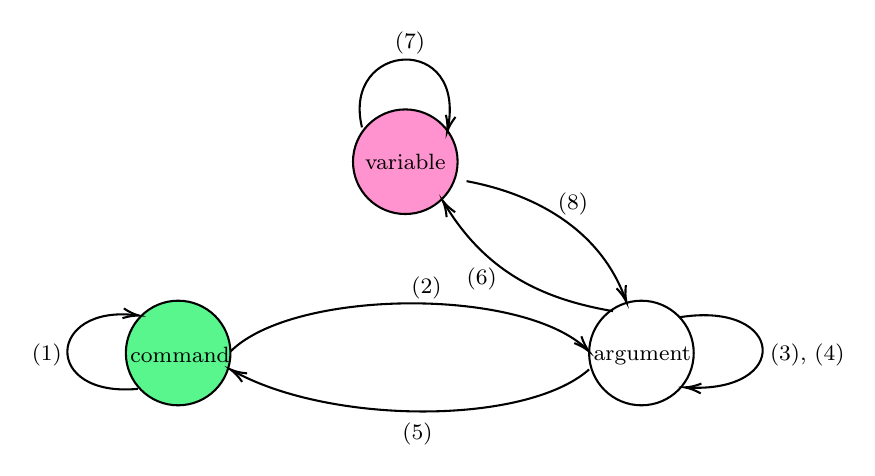
\begin{tikzpicture}[x=0.75pt,y=0.75pt,yscale=-0.72,xscale=0.72]
%Flowchart: Connector [id:dp006172763589022745] 
\draw  [fill={rgb, 255:red, 89; green, 246; blue, 142 }  ,fill opacity=1 ] (100,218) .. controls (100,198.67) and (115.67,183) .. (135,183) .. controls (154.33,183) and (170,198.67) .. (170,218) .. controls (170,237.33) and (154.33,253) .. (135,253) .. controls (115.67,253) and (100,237.33) .. (100,218) -- cycle ;
%Flowchart: Connector [id:dp9857393942850851] 
\draw   (410,218) .. controls (410,198.67) and (425.67,183) .. (445,183) .. controls (464.33,183) and (480,198.67) .. (480,218) .. controls (480,237.33) and (464.33,253) .. (445,253) .. controls (425.67,253) and (410,237.33) .. (410,218) -- cycle ;
%Curve Lines [id:da5249870829172163] 
\draw    (170,217) .. controls (212.09,174.95) and (365.4,173.55) .. (408.72,215.71) ;
\draw [shift={(410,217)}, rotate = 226.34] [color={rgb, 255:red, 0; green, 0; blue, 0 }  ][line width=0.75]    (10.93,-3.29) .. controls (6.95,-1.4) and (3.31,-0.3) .. (0,0) .. controls (3.31,0.3) and (6.95,1.4) .. (10.93,3.29)   ;
%Curve Lines [id:da1715846206115994] 
\draw    (410,229) .. controls (367.22,266.81) and (235.33,266.01) .. (170.97,229.55) ;
\draw [shift={(170,229)}, rotate = 30.03] [color={rgb, 255:red, 0; green, 0; blue, 0 }  ][line width=0.75]    (10.93,-3.29) .. controls (6.95,-1.4) and (3.31,-0.3) .. (0,0) .. controls (3.31,0.3) and (6.95,1.4) .. (10.93,3.29)   ;
%Flowchart: Connector [id:dp3515667087969462] 
\draw  [fill={rgb, 255:red, 255; green, 147; blue, 208 }  ,fill opacity=1 ] (252,90) .. controls (252,70.67) and (267.67,55) .. (287,55) .. controls (306.33,55) and (322,70.67) .. (322,90) .. controls (322,109.33) and (306.33,125) .. (287,125) .. controls (267.67,125) and (252,109.33) .. (252,90) -- cycle ;
%Curve Lines [id:da5437841267502748] 
\draw    (426,190) .. controls (379.47,182.08) and (340.78,164.36) .. (312.84,117.43) ;
\draw [shift={(312,116)}, rotate = 59.74] [color={rgb, 255:red, 0; green, 0; blue, 0 }  ][line width=0.75]    (10.93,-3.29) .. controls (6.95,-1.4) and (3.31,-0.3) .. (0,0) .. controls (3.31,0.3) and (6.95,1.4) .. (10.93,3.29)   ;
%Curve Lines [id:da24297836032951825] 
\draw    (328,103) .. controls (375.52,111.91) and (418.14,136.5) .. (434.51,182.6) ;
\draw [shift={(435,184)}, rotate = 251.2] [color={rgb, 255:red, 0; green, 0; blue, 0 }  ][line width=0.75]    (10.93,-3.29) .. controls (6.95,-1.4) and (3.31,-0.3) .. (0,0) .. controls (3.31,0.3) and (6.95,1.4) .. (10.93,3.29)   ;
%Curve Lines [id:da2798236433090334] 
\draw    (108,242) .. controls (43.65,247.94) and (46.93,185.27) .. (107.16,192.75) ;
\draw [shift={(109,193)}, rotate = 188.26] [color={rgb, 255:red, 0; green, 0; blue, 0 }  ][line width=0.75]    (10.93,-3.29) .. controls (6.95,-1.4) and (3.31,-0.3) .. (0,0) .. controls (3.31,0.3) and (6.95,1.4) .. (10.93,3.29)   ;
%Curve Lines [id:da15564769244860654] 
\draw    (258,67) .. controls (244.07,9.29) and (329.14,3.06) .. (315.22,69) ;
\draw [shift={(315,70)}, rotate = 282.62] [color={rgb, 255:red, 0; green, 0; blue, 0 }  ][line width=0.75]    (10.93,-3.29) .. controls (6.95,-1.4) and (3.31,-0.3) .. (0,0) .. controls (3.31,0.3) and (6.95,1.4) .. (10.93,3.29)   ;
%Curve Lines [id:da0016551100974000477] 
\draw    (471,194) .. controls (541.65,183.05) and (545.96,245.37) .. (475.07,241.07) ;
\draw [shift={(474,241)}, rotate = 3.97] [color={rgb, 255:red, 0; green, 0; blue, 0 }  ][line width=0.75]    (10.93,-3.29) .. controls (6.95,-1.4) and (3.31,-0.3) .. (0,0) .. controls (3.31,0.3) and (6.95,1.4) .. (10.93,3.29)   ;

% Text Node
\draw (101,212) node [anchor=north west][inner sep=0.75pt]   [align=left] {{\footnotesize command}};
% Text Node
\draw (411,212) node [anchor=north west][inner sep=0.75pt]   [align=left] {{\footnotesize argument}};
% Text Node
\draw (258,83) node [anchor=north west][inner sep=0.75pt]   [align=left] {{\footnotesize variable}};
% Text Node
\draw (35,210) node [anchor=north west][inner sep=0.75pt]  [font=\normalsize] [align=left] {{\footnotesize (1)}};
% Text Node
\draw (289,165) node [anchor=north west][inner sep=0.75pt]   [align=left] {{\footnotesize (2)}};
% Text Node
\draw (529,210) node [anchor=north west][inner sep=0.75pt]   [align=left] {{\footnotesize (3), (4)}};
% Text Node
\draw (283,263) node [anchor=north west][inner sep=0.75pt]   [align=left] {{\footnotesize (5)}};
% Text Node
\draw (387,109) node [anchor=north west][inner sep=0.75pt]   [align=left] {{\footnotesize (8)}};
% Text Node
\draw (326,159) node [anchor=north west][inner sep=0.75pt]   [align=left] {{\footnotesize (6)}};
% Text Node
\draw (278,1) node [anchor=north west][inner sep=0.75pt]   [align=left] {{\footnotesize (7)}};
\end{tikzpicture}
\caption{Simplified Version of the State Machine used for Command Parsing} \label{fig:shell_parser}
\end{figure}

Operating on a single character at a time, we handle the following transitions as part of the simplified command parsing (see Figure \ref{fig:shell_parser}):
\begin{itemize}
	\item \textbf{(1)}, \textbf{(3)}, \textbf{(7)} Read the current character and append it to the respective buffer, implemented as a \texttt{dynamic\_array}.
	\item \textbf{(2)} If the current character is a whitespace, we append the contents of the command buffer to the set of commands and start reading arguments.
	\item \textbf{(4)} A whitespace character denotes the end of an argument. Therefore, we append the contents of the argument buffer to the list of arguments, and begin parsing of the next argument.
	\item \textbf{(6)} If the current character denotes the beginning of a variable, i.e., equals \texttt{'\$'}, we treat successive characters as part of a variable.
	\item \textbf{(8)} Once the end of a variable has been detected, typically be a whitespace character, we look up the contents of the variable buffer in the trie storing active session variables.
	\item \textbf{(5)} If the current character represents an operator, e.g., \texttt{|}, \texttt{;}\footnote{For two character operators, e.g., \texttt{\&\&} and \texttt{||}, we may need to peek at the next character.}, it denotes the end of an argument list and the start of a succeeding command. Therefore, we append the current argument to the set of arguments of the current command and the operator to the list of operators.
\end{itemize}


Our implementation builds upon the simplified state machine, additionally checking for quoted strings and escape sequences as part of the \texttt{command} and \texttt{argument} states. As a result of performing this parsing stage, we obtain a parsed list of commands, including arguments and the delimiting operators. The parsed command line is stored in a \texttt{struct parsed\_command\_pipeline}:

\begin{lstlisting}[caption={Shell: Enabling Command History via the \texttt{history\_item} struct},label={listing:shell_parsed_cmd_pipeline}]
/// struct storing a single command within a pipeline
struct parsed_command {
    char  *command;
    size_t argc;
    char **argv;
};
/// entire parsed command pipeline, consisting of multiple commands
struct parsed_command_pipeline {
    size_t                 size;
    struct parsed_command *cmds;
    char                  *ops;  ///< (size-1) delimiting operators
    char                  *err_str;
};
\end{lstlisting}

\texttt{cmdparse.c}  also includes variations of the outlined function that support tab completion and syntax highlighting. However, from a conceptual standpoint, both procedures closely resemble the outlined methodology. The main difference lies in the actions carried out during each transition.

\subsection{Session Variables}\label{sec:shell_session_vars}

\newcommand{\ShellVar}[1]{{\color{shell_variable}\texttt{#1}}}

The shell automatically stores the PID (\ShellVar{\$!}) and the exit code (\ShellVar{\$?}) as variables when executing commands\footnote{\ShellVar{\$?} is only set when spawning applications in the foreground}. For any \emph{builtin}, the stored PID variable corresponds to the PID of the shell, whereas the \ShellVar{\$!} variable reflects PID of the spawn process in the case of an \emph{alias}. See section \ref{sec:shell_builtin} for the difference between the two.

In addition to implementing the required \ShellVar{\$?} and \ShellVar{\$!} variables, the shell supports arbitrary user defined variables. Variables are declared using \texttt{bash} syntax\footnote{Variables cannot be declared as part of a command, and must be declared a single variable at a time.}:

\begin{lstlisting}[style=ShellInputStyle]
 +~$+ @my_var@=42
 define: my_var := '42'
\end{lstlisting}

declares a variable named \texttt{my\_var} and sets its value to $42$. After having defined the variable, it can be used via the \ShellVar{\$my\_var} syntax:


\begin{lstlisting}[style=ShellInputStyle]
 +~$+ echo "my_var has the value @$my_var@"
 my_var has the value 42
\end{lstlisting}

Currently, it is not possible to declare variables as part of a command, or to declare multiple variables in a single line.

Internally, all active session variables are stored in a trie. This allows variables to be inserted/updated efficiently, while simultaneously serving as the foundation for their tab completion.

\begin{figure}[htp]
    \centering
    \includegraphics[width=6.5cm]{images/shell/var_trie.png}
    \caption{Trie Storing Active Session Variables}
    \label{fig:shell_var_trie}
\end{figure}

Note that variables are substituted as part of the \emph{parsing stage}. This implies that the following are semantically different:

 \begin{lstlisting}[style=ShellInputStyle]
 +~$+ run hello
 +~$+ echo @$!@
\end{lstlisting}

runs the \texttt{hello} application and outputs its process identifier (PID), whereas

 \begin{lstlisting}[style=ShellInputStyle]
 +~$+ run hello +;+ echo @$!@
\end{lstlisting}

runs the \texttt{hello} application and outputs the preceeding process' PID, i.e., the one we would have obtained by running \texttt{echo \$!} directly.

\begin{comment}
	maybe think about mentioning that they are "implicitly quoted" (i.e., count as a single argument) 
\end{comment}

\subsection{Syntax Highlighting}\label{sec:shell_syntax_highlighting}

Syntax highlighting in a shell is essential as it enables users to visually differentiate elements within a single line of input, such as commands, variables, and operators. This distinction significantly improves productivity and enhances the user experience. Similar to tab completion, syntax highlighting builds upon a specialized variant of the parsing stage, in this case: \texttt{\_pst\_color\_char}.

As part of the aforementioned function, the shell populates a \href{https://en.wikipedia.org/wiki/Dynamic_array}{\texttt{dynamic\_array}} of \texttt{cmdline\_color\_t}s. Each \texttt{cmdline\_color\_t} constitutes of a starting position \texttt{begin} and a buffer storing the color to apply, encoded using \href{https://en.wikipedia.org/wiki/ANSI_escape_code}{ANSI escape codes}. When refreshing the current line, the shell respects the constructed array of colors, by applying them in the correct order. As supporting syntax highlighting requires additional line refreshes, it is possible to disable syntax highlighting via the corresponding \texttt{SHELL\_CMDLINE\_COLORS} macro.

\begin{lstlisting}[style=ShellInputStyle]
 +~$+ echo "syntax %*\shellquote* highlighting @$rocks@" +>+ §out.txt§
\end{lstlisting}

As every character potentially requires a line refresh with syntax highlighting, we experimented with refreshing the line on every input. This occasionally causes blinking. Thus, in the current implementation the shell refreshes the line only upon processing \emph{special characters}, e.g.,  whitespaces and  operators.


\section{Shell Builtins} \label{sec:shell_builtin}

Thoughtful consideration has been given to designing the way command are defined in order to facilitate the implementation of a wide range of functionalities within the shell. The excerpt of \texttt{cmdbuiltins.h} shown in Listing \ref{listing:shell_cmd_define} explains how commands are defined within the shell. Specifically, defining commands as part of the macro ensures that they are listed in the \texttt{help} command, the corresponding \texttt{man} pages are populated, and that the commands are inserted into the command trie.

\begin{lstlisting}[caption={Shell: Defining \texttt{BUILTIN}s and \texttt{ALIAS}es as Part of the Shell},label={listing:shell_cmd_define}]
#define CMD_BUILTIN_FOREACH(BUILTIN, ALIAS) 	                 \
   BUILTIN(man, CMD_BUILTIN_GROUP_BASIC, _cmd_builtin_man,     \
	         "display a manual pages", "man <builtin>", NULL)    \
   ALIAS(echo, CMD_BUILTIN_GROUP_BASIC,                        \
         "writes the first argument to standard output",       \
         "echo <message>", "[...]")                            \
   [...]\end{lstlisting}

For an exhaustive list of all implemented commands, we refer to the User Guide of Appendix Section \ref{sec:appendix_user_guide}.

As Listing \ref{listing:shell_cmd_define} indicates, the shell differentiates between \emph{builtin}s and \emph{alias}es. A builtin is executed \emph{as part of} the shell, whereas an \emph{alias} is delegated to a seperate process.  For example, executing the alias \texttt{echo} can be considered equivalent to executing \texttt{run echo}.

In most cases, this distinction is not visible to the user. For \emph{command pipelines}, as discussed in section \ref{sec:shell_pipes_and_io}, this difference is important. In particular, any command defined as a builtin cannot appear as part of a command pipeline\footnote{\texttt{BUILTIN}s may still appear within a list of commands.}. This limitation is a result of the way I/O redirection is implemented: we would have to redirect the shell's input/output, or handle this case explicitly.

\begin{comment}
	TODO: mention launching a "shell within a shell"
\end{comment}

\subsection{The \texttt{time} Utility}

The \texttt{time} utility measures the time taken to execute another command. As we want to support timing the execution of command pipelines and list of commands, \texttt{time} is neither implemented as a \texttt{BUILTIN} nor as an \texttt{ALIAS}\footnote{Technically speaking, we provide a \texttt{time} builtin for the purpose of detecting illegal use, populating \texttt{help}, and the corresponding \texttt{man} page.}. Instead, the shell explicitly checks if the parsed list of commands starts with a \texttt{time} directive. In this case, the shell initiates timed execution of the entire set of commands, as depicted in Listing \ref{listing:shell_time_ex}.

\begin{lstlisting}[style=ShellInputStyle, caption={Timing the Execution of a List of Commands}, deletekeywords={echo, command}, label={listing:shell_time_ex}]
 +~$+ time echo "first command" +;+ !echo! "second command"
 first command
 second command
 %took: 0m:0.218s% (real)
\end{lstlisting}

\subsection{Process Management}

The shell provides numerous commands to allow the user to effectively manage processes, e.g., \texttt{kill}, \texttt{pause}, \texttt{resume}, and \texttt{ps}. Most importantly, however, the shell facilitates spawning processes via the \texttt{run <command> [\&]} and \texttt{oncore <core\_id> <command> [\&]} builtins. 

Both builtins spawn the requested process in the foreground by default, and support spawning the background via an optional trailing \texttt{\&}. Additionally, \texttt{oncore} supports spawning a process on a specific core, as specified via the required \texttt{core\_id} argument.


Spawning a process in the foreground is rather straightforward. The shell simply calls \texttt{proc\_mgmt\_spawn\_program\_argv}\footnote{Technically, it uses a variant discussed in subsequent chapters.} to spawn the process with the parsed parameters and sets \ShellVar{\$!}. Subsequently, it waits for completion of the newly spawn process by invoking \texttt{proc\_mgmt\_wait}. At this point, it is able to set the resulting \ShellVar{\$?} variable.

In contrast, spawning a process in the background is slightly more complex. The shell cannot wait for termination, and thus does not set the  \ShellVar{\$?} variable. Additionally, the shell must prevent the spawned application from consuming console input. Building upon the infrastructure set in place to support I/O redirection, the shell does this by mapping an empty frame as the process' standard input, while preserving its standard output. This means that any application spawned in the background may still print to the console as expected. Specifics related to the implementation of \emph{overriding} a process' standard in- and output are detailed in section \ref{sec:shell_pipes_and_io}.

\subsection{Filesystem}


The filesystem, a fundamental component of any operatating system, is crucial for organizing, storing, and accessing data. The shell uses this component to facilitate effective file management and navigation.

The shell stores the working directory as part of the current session. This allows builtins to operate on relative, as opposed to solely absolute, paths. To support relative paths within \texttt{ALIAS}es, the shell supplies the current working directory via a dedicated \texttt{-\phantom{}-wd} flag when spawning the associated process.

In the upcoming section, it will become evident that the shell heavily relies on the versatile \texttt{tee} alias/program to facilitate I/O redirection to files. By accepting multiple file names as command line arguments, \texttt{tee} effectively duplicates its standard input to those files.  Moreover, when \texttt{tee} is executed without the \texttt{-s} option, it further prints its standard input to the standard output (\texttt{stdout}).

To enhance functionality, we offer support for automatically suggesting file and directory names within the current directory as an experimental feature. To activate this feature, you can enable the \texttt{SHELL\_TAB\_COMPLETE\_FILENAMES} macro in the \texttt{shell.h} file.

\section{Extra Challenge: Pipes and I/O Redirection} \label{sec:shell_pipes_and_io}

While it is already useful to spawn an individual process, the use of the shell becomes substantially more effective when it starts to orchestrate sets of command pipelines. In particular, \href{https://en.wikipedia.org/wiki/Pipeline_(Unix)}{Unix Pipelines} offer a highly valuable abstraction for this purpose. In the following, we explore the implementation of command pipelines and their role in constructing \emph{lists of commands}.
\subsection{Command Pipelines}

A pipeline is a powerful concept in which processes are interconnected, forming a chain through their standard input and output streams. This arrangement allows the output of each process (\texttt{stdout}) to be seamlessly passed as input (\texttt{stdin}) to the next process. It is important to note that all the processes within a pipeline are executed concurrently, thereby enhancing efficiency and enabling faster execution. Listing \ref{listing:shell_pipeline_ex} provides an example of a pipeline evaluation.

\begin{lstlisting}[style=ShellInputStyle, deletekeywords={command}, caption={Execution of an Exemplary Pipeline}, label={listing:shell_pipeline_ex}]
 +~$+ echo "something to pipeline across process'" | wc
       1       5      38
\end{lstlisting}

The shell also supports redirecting a process' output via \texttt{>}. To unify both types of redirection any use of \texttt{>} is \emph{desugared}, making use of the \texttt{tee} alias. E.g., the statement

\begin{lstlisting}[style=ShellInputStyle, deletekeywords={command}]
 +~$+ echo "my very long string" +|+ wc -l +>+ §foo.txt§
\end{lstlisting}
is translated into
\begin{lstlisting}[style=ShellInputStyle, deletekeywords={command}]
 +~$+ echo "my very long string" +|+ wc -l +|+ tee foo.txt -s
\end{lstlisting}

wherein the trailing \texttt{-s} is appended in case the respective file redirection is the last command within the current pipeline. Otherwise, it is omitted. This allows pipelines to contain multiple successive file redirections, e.g.,
\begin{lstlisting}[style=ShellInputStyle, deletekeywords={command}]
 +~$+ echo "very important message" +>+ §file1.txt§ +>+ §file2.txt§
\end{lstlisting}
or after \emph{desugaring}
\begin{lstlisting}[style=ShellInputStyle, deletekeywords={command}]
 +~$+ echo "very important message" +|+ tee file1.txt +|+ tee file2.txt -s
\end{lstlisting}
in which case both \texttt{file1.txt} and \texttt{file2.txt} will be populated. This follows naturally, as \texttt{tee} additionally replicates its input to \texttt{stdout} if \texttt{-s} is ommited. Thus, the second \emph{desugared} \texttt{tee} will be passed the duplicated input.

After \emph{desugaring}, the shell must, therefore, only facilitate the seamless flow of standard streams through a series of successive processes. This functionality is built on top of User-Level Message Passing (UMP). To enable pipelines, the following generalization of \texttt{spawn\_load\_with\_caps} was introduced:

\begin{lstlisting}[caption={Generalization of \texttt{spawn\_load\_with\_caps}}]
errval_t spawn_load_mapped(struct spawninfo *si,
	struct elfimg *img, int argc, const char *argv[], int capc,
	struct capref caps[], domainid_t pid, struct capref stdin_frame,
	struct capref stdout_frame);\end{lstlisting}

While accepting mostly the same arguments as \texttt{spawn\_load\_with\_caps}, the caller is able to provide additional \texttt{stdin\_frame} and \texttt{stdout\_frame} parameters. These frames are emplaced into the newly constructed process' \texttt{CSpace} at well-known locations: \texttt{TASKCN\_SLOT\_STDIN\_FRAME} and \texttt{TASKCN\_SLOT\_STDOUT\_FRAME} respectively.

Both slots are checked as part of the thread initialization performed in \texttt{barrelfish\_init\_onthread}. If the slots are populated appropriately, a UMP endpoint is initialized using the passed frame. Subsequent reads/writes now make use of the corresponding UMP functions. If a frame is not initialized, reads/writes rely on the standard rpc functionality as described in section \ref{sec:shell_io_via_rpc}. This logic is encapsulated in the \texttt{iox} library. The libc function pointers are set up to make use of this abstraction:

\begin{lstlisting}[caption={}]
_libc_terminal_read_func  = iox_read;
_libc_terminal_write_func = iox_write;\end{lstlisting}

To orchestrate a pipeline, the shell makes use of the rpc \emph{wrapper} of this function, \texttt{aos\_rpc\_proc\_spawn\_mapped}. First, the shell allocates a sufficient number of frames\footnote{For a pipeline of length $n$, the shell allocates $n - 1$ frames.} and then spawns the requested programs, providing the corresponding in- and output frames. This mapping is visualized in Figure \ref{fig:shell_pipes}. After having spawned all processes, the shell waits for their completion.

\begin{figure}[htp]
    \centering
    \includegraphics[width=12cm]{images/shell/shell_pipes.png}
    \caption{Pipeline orchestrated by the Shell}
    \label{fig:shell_pipes}
\end{figure}

The way pipelines are constructed, any command that is part of a pipeline\footnote{of size at least two} must be an \texttt{ALIAS} and not a \texttt{BUILTIN}. As any command within the pipeline must, consequently, refer to a separate program, the user may omit the \texttt{run} / \texttt{oncore} tokens\footnote{However, it remains perfectly valid to keep them}. This is illustrated in Listing \ref{listing:shell_pipeline_omit}.

\begin{lstlisting}[style=ShellInputStyle, deletekeywords={run, command, wc, echo}, caption={Pipelines with or without the \texttt{run}/\texttt{oncore} Directives}, label={listing:shell_pipeline_omit}]
 +~$+ !run! echo "commands can be executed with run" | !run! wc -l
      1       6      34
 +~$+ !echo! "commands can be executed without run" | !wc! -l
      1       6      37
\end{lstlisting}

Furthermore, the operating system supports sending capabilities across cores, as detailed in chapter \ref{chapter:distcap}. Therefore, pipelines can naturally be used to facilitate arbitrary communication between processes across cores:

\begin{lstlisting}[style=ShellInputStyle, deletekeywords={run, command, wc, echo}]
 +~$+ !oncore! 1 echo "hello from the other core..." | !oncore! 0 wc
      1       5      29
\end{lstlisting}


 Note that a process can still perform explicit printing and reading operations to the terminal using the corresponding RPC calls. We discussed the possibility of introducing a permission system, allowing processes to be spawned with a limited set of permitted operations. However, in the end, we chose not to implement such a mechanism.

\subsection{Lists of Commands}

Similar to bash, our shell supports \href{https://www.gnu.org/software/bash/manual/html_node/Lists.html}{Lists of Commands}. A list of commands consists of one or more pipelines arranged in a specific order, with each pipeline separated by one of the following operators: \texttt{;}, \texttt{\&\&}, or \texttt{||}. 

Mutliple pipelines within a list of commands are not run concurrently. Instead, pipelines are executed sequentially one after another, potentially short-circuiting based on the exit code:
\begin{itemize}
	\item \texttt{;} No short-circuiting is applied. The exit code corresponds to the last executed command pipeline.
	\item \texttt{\&\&} If the previous pipeline returned an exit code \texttt{!= 0}, execution ends immediately, returning the preceding pipeline's exit code
\begin{lstlisting}[style=ShellInputStyle, deletekeywords={run, command, wc, echo}]
 +~$+ true +&&+ !echo! "short-circuiting example"
 short-circuiting example
 +~$+ false +&&+ !echo! "short-circuiting example"
\end{lstlisting}
	\item \texttt{||} If the previous pipeline returned an exit code \texttt{== 0}, execution ends immediately, with the exit code $0$.
\begin{lstlisting}[style=ShellInputStyle, deletekeywords={run, command, wc, echo}]
 +~$+ true +||+ !echo! "short-circuiting example"
 +~$+ false +||+ !echo! "short-circuiting example"
 short-circuiting example
\end{lstlisting}
\end{itemize}

Futhermore, pipelines are always executed from left to right, i.e., all operators delimiting pipelines \texttt{;}, \texttt{\&\&}, \texttt{||} have the same operator precedence. This significantly simplifies parsing, while adhering to the bash specification. Currently, there is no way to group commands.

\section{Limitations}

As described in the previous sections, the shell supports a large number of features, from syntax highlighting and tab completion to I/O redirection and pipes. Building upon the existing capabilities, there are several potential avenues to further improve the functionality of the shell:
\bigbreak
\textbf{Interleaving between \texttt{debug\_printf} and \texttt{printf}} Debug output printed as part of a \texttt{debug\_printf} may be interleaved with output of the serial server. This is a consequence of \texttt{debug\_printf} relying on the corresponding \texttt{SYSCALL}, which in turn accesses the UART driver directly. To prevent such an interleaving, we may call the serial server for \texttt{debug\_printf}, or write debug output to a dedicated file.
\bigbreak
\textbf{Improved Syntax Highlighting} The current version of syntax highlighting could be extended to correctly display the \texttt{time} primitive, to highlight the command argument passed to \texttt{run}/\texttt{oncore}, or to highlight files.
\bigbreak
\textbf{Support for \texttt{BUILTIN}s in Command Pipelines} One limitation of our command pipelines is that they do not support running \texttt{BUILTIN}s. Instead, only an alias/binary may be run from within a pipeline. It may be worthwhile to consider adding support \texttt{BUILTIN}s, by spawning them in a separate process, or by having the shell populate the relevant I/O frames.
\bigbreak
\textbf{Tab completion for Command Arguments} Tab completion for command arguments is already supported in theory, as demonstrated by the support for auto-completing filenames. In addition, it could be implemented for the most common \texttt{BUILTIN}s/\texttt{ALIAS}es. In particular, we may consider implementing tab completion for the first argument of \texttt{run}, i.e., the program to execute.
\bigbreak
\textbf{Permissions for Mapped Processes} In our current implementation, any process is able to print and read from the terminal via the UART by explicitly calling the corresponding RPC calls. One might extend our solution by implementing a permission system, so that this is no longer possible.
\bigbreak
\textbf{General Purpose Working Directory} Instead of using the \texttt{\-\phantom\-wd} flag to provide the current working directory when launching a process associated with an alias like \texttt{ls} or \texttt{tee}, an alternative approach could be to offer a general purpose function to retrieve the current working directory. This would enable processes to access and retrieve the working directory when they are launched using \texttt{run} or \texttt{oncore}. 

\section{Retrospective}

Working on this milestone was a challenging and simultaneously rewarding journey. By implementing the entire shell from the ground up, I have considerably improved my understanding of the whole stack: from the intricacies of dealing with I/O, as part of \texttt{readline} and implementing fundamental data structures such as tries and gap buffers, to the efficient transfer of data between processes using piping.

As this task took considerable amounts of time, sweet, and tears, I would \emph{certainly} recommend to instead port the readline code from \texttt{FreeBSD} libraries, as helpfully pointed out in the book.